\subsection{Glasfaser}
Glasfasern gelten als älteste synthetische Faserart und wurden schon vor 3500 Jahren verwendet. Heute werden Glasfasern überwiegend aus SiO2 und Metalloxiden hergestellt. Die Bestandteile werden bei ca. 1400°C aufgeschmolzen und durch kleine Düsen im Boden des Kessels als dünne Fäden ausgelassen. Die Fäden werden aufgewickelt und zu größeren Fasern versponnen (vgl. \cite{item3})
Die hohe Festigkeit der Glasfaser beruht auf den kovalenten Bindungen von Silizium- und Sauerstoff-Atomen. Zugesetzte Metalloxide verhindern eine Ausbildung eines geordneten Gefüges und erhöhen somit zusätzlich die Festigkeit. Die Fasern können in Längsrichtung sehr hohe Kräfte aufnehmen, jedoch nicht in Querrichtung. Deshalb werden sie in eine Matrix integriert, die die Querkräfte aufnimmt und die Faser vor dem Knicken schützt. Glasfasern lassen sich auch um enge Radien sehr gut drapieren und sind durch ihre einfache Herstellungsweise sehr preiswert [4].
Durch die zuvor erläuterten Eigenschaften sind Glasfasern sehr gut für dieses Projekt geeignet, für einen größeren Flügel wäre jedoch der Elastizitätsmodul zu gering und es müsste auf andere Fasern, wie zum Beispiel Kohlefasern zurückgegriffen werden. 
Für die Konstruktion des Flügels stehen die Glasfasern Interglas 90070 und Interglas 92145 des Herstellers Interglas Technologies zur Verfügung. 

\subsection{Matrix}
Unter der Matrix versteht man den die Fasern umgebenden Teil des Faserverbundstoffs. Dabei werden im Bereich des Faser-Kunststoff-Verbunds Polymere wie z.B. Epoxidharz verwendet. Die Matrix ist meist der schwache Teil des FKV und ist dafür da um die Fasern gegen Knicken bei Druckbelastung zu schützen und eine gleichmäßige Krafteinleitung in die Fasern zu ermöglichen. Zusätzlich hält sie die Fasern in Position und verhindert Reibung zwischen den einzelnen Fasern.\\  Weiterer Text folgt.
\subsection{Netztheorie}
Text folgt noch, hiermit soll jedoch nicht gerechnet werden.
\subsection{Klassische Laminattheorie}
Text folgt noch
\subsection{Versagenskriterium nach Puck}
Text folgt noch
\subsection{Bauweise}
In der Aufgabenstellung wird gefordert, dass der Flügel in der Holm-Bauweise konstruiert wird. Ein Holm besteht aus zwei parallelen Gurten, die durch einen oder mehrere Stege miteinander verbunden werden. Dabei sind verschiedene Varianten möglich. Abbildung ~\ref{fig: Holmarten} veranschaulicht Konstruktionsmöglichkeiten. Neben der Festigkeit ist die Steifigkeit die einzige strukturmechanische Anforderung. Somit lässt sich das Problem als Biegebalken betrachten, der bei der vorgegebenen Prüflast $ F_{pruef}=100N $ am freien Ende die vorgegebene Durchbiegung $ w(100N)=22mm $ einhält. Das entstehende Biegemoment wird hauptsächlich von den Gurten getragen, weswegen man sich bei der Wahl des Steges auf andere Kriterien konzentrieren kann. Da kein maximaler Drillwinkel vorgegeben ist und die Torsionssteifigkeit fast ausschließlich von der Haut bewirkt wird, führen mehrere Stege, wie man sie bei einem geschlossenen Profil hat, nur zu unerwünschter Gewichtszunahme. Nach diesen Überlegungen wurde der I-Holm ausgewählt, da dieser bei einfacher Fertigung die gewünschten Eigenschaften mit sich bringt.
\begin{figure}
	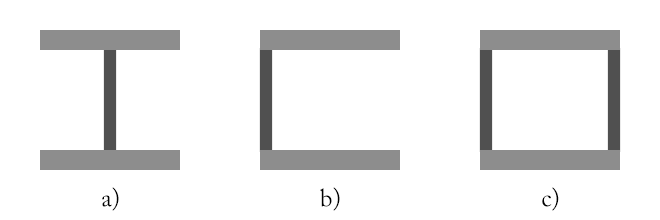
\includegraphics[width=1.0\textwidth]{Bilder/Holmarten.png}
	\caption{a) I-Holm   b) C-Holm    c) Kastenholm}
	\label{fig: Holmarten}
\end{figure} 
Das aerodynamische Profil des Flügels wird durch Schalenbauweise erreicht. Hierbei wird eine dünne Haut nur an kritischen Stellen mit der Sandwichbauweise beziehungsweise Rippen an den kritischen Stellen verstärkt, um Beulen zu verhindern. Die Schale trägt dabei so gut wie gar nicht die Last des Flügels, jedoch ist sie für die Torsionssteifigkeit entscheidend.
